%----------------------------------------------------------------------------------------
%	PACKETS AND CONFIGURATION
%----------------------------------------------------------------------------------------

\documentclass{beamer}

% \usepackage{tikz} \usepackage{pgfplots} \usepackage{graphicx} % for graphs

\usepackage{title}  % Title settings for the presentation

\usetheme{Copenhagen} % THEME

%----------------------------------------------------------------------------------------
%	DOCUMENT
%----------------------------------------------------------------------------------------

\begin{document}

% TITLE
\frame{\titlepage}

% Table of Contents
\begin{frame}{Project}
    \tableofcontents[hideallsubsections]
\end{frame}

% Environment and Simulation ------------------------------------------------------------

\AtBeginSection[]
{
\begin{frame}{}
    \tableofcontents[currentsection]
\end{frame}
}

% ----------------------------------------

\section{Environment and Simulator}

\begin{frame}{Fully justified}

\frametitle{Environment and Simulator}
\framesubtitle{Environment}
The environment is modelled to give as output a class cointaing all the sample values for a day of interaction for each users class.
Single arguments of the class can be specified, if desired, also to test the algorithms in limits case.

\end{frame}

% ----------------------------------------

\begin {frame} {Fully justified}

\frametitle{Environment and Simulator}
\framesubtitle{Randomness}
To better compare the results and more importantly having a real scenario all the parameters not known a priori are randomnly generated.
More over there is the possibility both to specify the random seed generator and to make the Environment and the Simulation deterministic, in order understand and check the performance of each learner.

\end {frame}

% ----------------------------------------

\begin{frame}{Fully justified}

\frametitle{Environment and Simulator}
\framesubtitle{Environment}
Through the environment we can set values that define univocally:
\vspace{0.5cm}
\begin{list}{-}{\setlength{\itemsep}{0.5cm}}
    \item Users'class and their Interaction with the website.
    \item The total amount of budget to subdivide.
    \item The ratios in which every class appears in the population.
    \item The prices of each product.
    \item The budget the competitor spends in advertising
\end{list}

\end {frame}

% ----------------------------------------

\begin {frame}{Fully justified}

\frametitle{Environment and Simulator}
\framesubtitle{Users class}
Each Users class is modelled with:\textbf{ reservation price, steepness, shift and upper bound}
for each product, including the one of the not strategic competitor.
Since the $alpha$-functions we had choosen belong to the sigmoidal class we need these additional parameters.

\begin{figure}[⟨b⟩]  
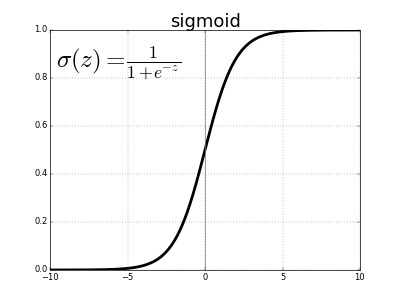
\includegraphics[height=4cm]{img/sigmoid.png}
    \end{figure}
\end {frame}

% ----------------------------------------

\begin {frame}{Fully justified}

\frametitle{Environment and Simulator}
\framesubtitle{Simulator}
Interacting with the environment it computes the margin made each day, for each of the different classes of users as an integer representing the total aggregated reward of the entire list of interactions.

\end{frame}

% ----------------------------------------

\begin {frame}{Fully justified}

\frametitle{Environment and Simulator}
\framesubtitle{Simulator}
It is also possible to create a "masked" environment which allows to test the different algorithms according to the data given at each step. Moreover it allows us to fed the clayrvoiant alghoritm with the same set of data, but not masked, for a better comparison.

\end{frame}

% Optimization Algorithm ----------------------------------------------------------------

\AtBeginSection[]
{
\begin{frame}{}
    \tableofcontents[currentsection]
\end{frame}
}

% ----------------------------------------

\section{Optimization Algorithm}

\begin{frame}{Fully justified}

\frametitle{Optimization Algorithm}
\framesubtitle{Problem Formulation}
Our aim is finding the optimal budget per campaign in order to maximize the profit.
which is defined as the difference between the expected margin and the spent in advertising
Basically, it is a maximisation subject to the obvious constraint: the sum of the daily budget can't be greater then the overall budget.

The optimization problem can be expressed as follows:
\begin{displaymath}
F=\max_{\substack{x_i\in B}} \sum_{i=0}^n \alpha_i(x_i)p_i-x_i \ s.t. \sum_{i=0}^n x_i\leq B
\end{displaymath}

\end{frame}

% ----------------------------------------

% Uncertain alpha functions -------------------------------------------------------------

\AtBeginSection[]
{
\begin{frame}{}
    \tableofcontents[currentsection]
\end{frame}
}

% ----------------------------------------

\section{Uncertain alpha-functions}

\begin {frame}{Fully justified}

\frametitle{Uncertain alpha-functions}
Since the feature of the users are \textbf{not osservable}, the algorithm take as input the aggregated list of interactions.
It tries to estimate the aggregated $alpha$-function and the reward of each single product

\end{frame}

% ----------------------------------------

\begin {frame}{Fully justified}

\frametitle{Uncertain $alpha$-functions}
\framesubtitle{Result}
% TODO: going to insert some graph of clayrvoiantv stupid v ts v ucb1

\end{frame}

% Uncertain alpha functions and number of items sold ------------------------------------

%\section{Uncertain $alpha$-functions and number of items sold}

% Uncertain graph weights ---------------------------------------------------------------

%\section{Uncertain Graph Weights}

% Non-stationary demand curve -----------------------------------------------------------

%\section{Non-stationary demand curve}

% Context generation --------------------------------------------------------------------

%\section{Context generation}

\end{document}
